\BiChapter{神经网络的设计技巧}{trick}
神经网络的设计技巧众多,这些技巧大致可分为两大类,一类是训练前对数据的预处理,另一类是训练过程中采用的一些特殊的训练手段。数据预处理的作用在于将原始数据处理成容易训练的数据,加快准则函数的收敛速度,另一方面,原始数据的降维可以在牺牲较小精度的前提下减少运算量,提高程序的执行效率。训练过程中采用的一些特殊手段在数学上是没有太大意义,甚至有时候是违反直觉的,这些技巧是多年来科研人员积累出来的经验,其灵感来源一般靠蒙。尽管这些经验有时候反而会降低网络的性能,但大部分情况下确实会提高性能的,某些情况下,不适用这些技巧,网络的训练初始阶段准则函数无法收敛。具体设计过程中,对于这些技巧,我们应该抱着试一试的心态,如果在网络中使用某个技巧,使得网络性能变好了,那么我们便保留这个技巧,否则如果网络性能变差了,那么就舍弃这个技巧\footnote{但前提是这个技巧被正确使用,即编码正确}。
\BiSection{数据预处理}
x数据的预处理大致可分为几类:白化、降维、扩容、归一化。白化的作用在于去除数据耦合的相关性,降维的作用在于压缩数据,加快算法执行效率,由于主成分分析是一种去除相关性的降维方法,因此我们将白化合并到主成分分析的章节中而不另起章节。扩容目的在于利用一些手段,人工地伪造一些训练数据,将训练样本的容量扩大,使得网络的泛化能力变强。归一化的目的在于让数据保持在$[0,1]$区间内,之所以要在这个区间内,一方面,在一些激活函数,比如Sigmoid函数中,如果数据尺度过大,则使得激活函数迅速饱和,从而梯度接近于0,权值更新缓慢。而数据归一化到较小的数值上时,我们知道,Sigmoid函数在原点附近是一个近似于线性的函数,在训练的初始阶段便可让权值获得较大的梯度。另一方面,如果数据尺度过大,有可能会导致计算机的数值溢出,尤其是激活函数为Sigmoid的时候,因为这个激活函数带有一个指数项,对于某些不自带溢出检测的编程语言如C++而言,这是一场灾难,因为它会导致你的代码莫名其妙地失败。即使是一些带溢出检测的语言,如Python,当数值溢出时,往往使用Inf或NaN代替,此时进行的不再是数值运算,而是符号运算,这将极大地降低运算速度。
\BiSubsection{降维}
x人是一种受限于三维空间的动物,我们只能理解三维的而无法想象更高维度的事物。事实上,人同样无法理解二维的或一维的世界,尽管我们可以在脑海中想象二维曲面或一维曲线,但人脑海里的这些事物这些都不是二维,他们只是嵌在三维空间中的二维(或一维)流形\footnote{更多有意思的观点可以观看麻省理工学院的《量子力学》公开课}。一张一百万像素的图片,它总能对应着一百万维空间中的某一点,而很多张某个类比的图片,比如狗的图片,将会对应着一百万维空间中的多个点。然而并不是一百万维空间中的任何一点都是狗的图片,它也有可能是猫的图片,但是同样是狗的图片,它会在总会有某些共通性,这些共通性,或者说特征,使得狗这一类图片在一百万维的空间中构成一个流形,如果我们能找到这个流形,那么我们就可以避开一百万维空间,直接在低维流形中进行分类。

由于我们无法理解高维空间,因此我们通过一个三维空间中的二维流形简单叙述这件事,如果我们通过式\eqref{equ:xyzpoint}求取三维空间中任何一点的$(x, y, z)$坐标
\begin{equation}
\alpha = 1.5\pi *(1+2 * random)
\end{equation}
\begin{equation}
x = \alpha * \cos\alpha~~~~~~~~y = 21 * random~~~~~~~~z = \alpha * \sin\alpha
\label{equ:xyzpoint}
\end{equation}
式中,$random$是$[0,1]$区间内均匀分布的随机数,那么我们就可以得到一个称为“swiss roll”的散点图,如图\ref{img:swiss roll}所示
\begin{figure}[!htbp]
\centering
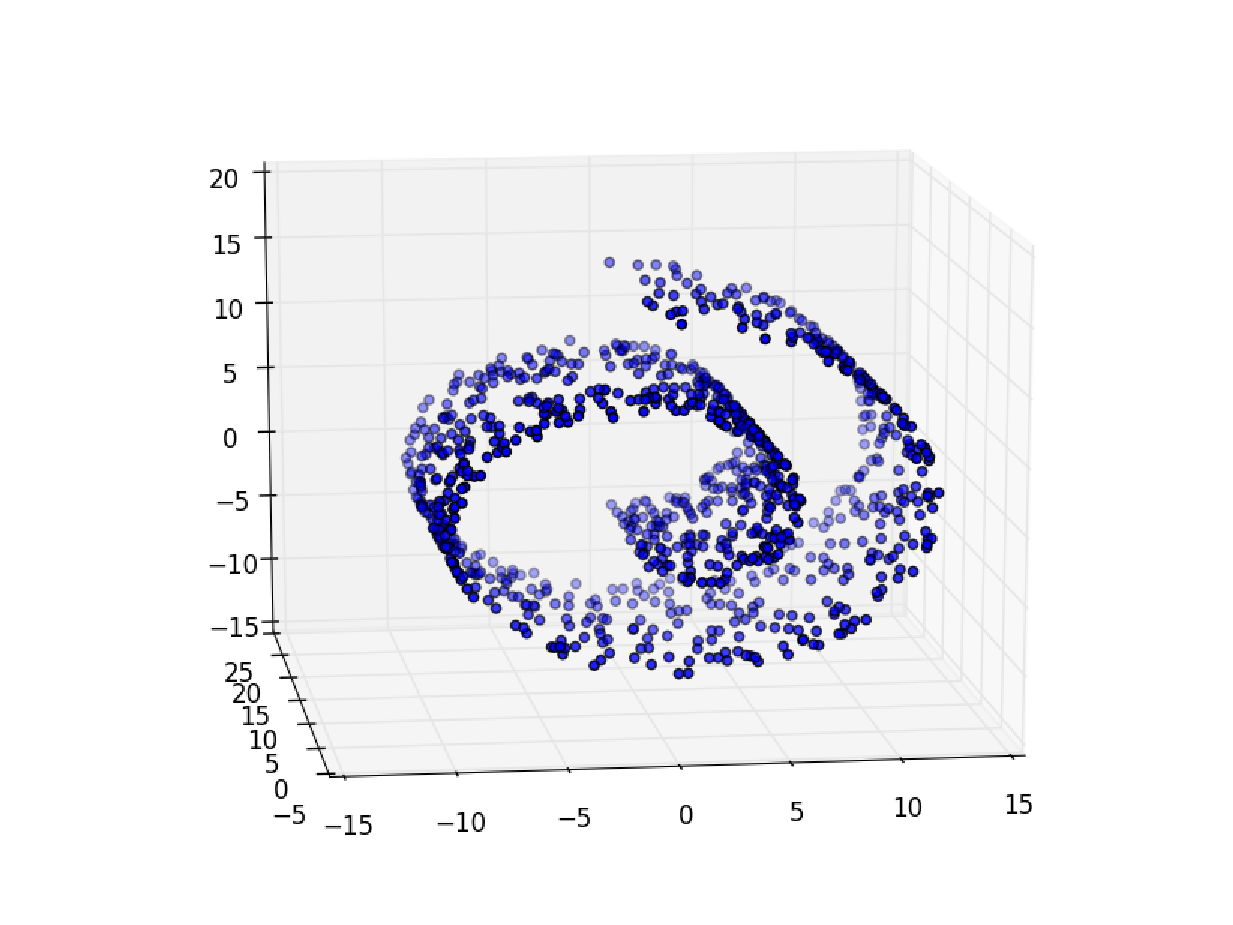
\includegraphics[width=0.8\textwidth]{trick/swissRoll.eps}
\caption{Swiss Roll}
\label{img:swiss roll}
\end{figure}
如果这些点分别代表一个三维的数据样本,那么我们可以发现,这些样本坐落于一个二维流形中,即图\ref{img:swiss roll}中卷筒蛋糕的形状。这里我们用了错误的措辞,因为流形实际上是一个空间而不是一个形状,但为了通俗地解释这件事,我们认为采用这种措辞是可取的。观察式\eqref{equ:xyzpoint},我们可以发现,事实上三维空间中的点$(x,y,z)$可以只用二维空间的$(\alpha, y)$描述,因为$x$和$z$都是$\alpha$的函数,从图像上我们也可以直观的感受到,三维数据是多余的,因为数据的坐落位置十分有规律。

降维,也是同样的思想,高维的数据是带有冗余的,如果我们能找到这些数据的低维流形,那么就可以在低维空间中进行数据处理。这衍生出了机器学习的一个流派---流形学习。关于流形学习我们不会做过多的介绍,我们只在本章中介绍两种降维方法,即主成分分析和多维尺度分析。与统计学习类似,实际中我们也无法找到数据真实的低维流形,不同的降维方法相当于对低维流形的不同逼近方法。如果说数据背后确实存在一个低维流形,而我们的降维方法又恰好是这个流形的描述,那么降维不会引入信息的损失,例如,三维坐标降到球坐标并不会引入误差,但实际中我们我们并不知道具体流形,我们的降维方法也不是真实的维度变换方法,所以实际中的降维一定会引入信息的损失,导致分类性能的下降,相比于降维带来的巨大好处----运算效率的提高,这个性能的下降是可接受的。图像识别,由于生活图像其维度都以千万记,降维是必须的,否则以目前的计算机性能无法完成准则函数的收敛。

\BiSubsubsection{主成分分析}
x为了简单起见,我们只在这里讨论如何使用主成分分析将二维空间中的数据降到一维空间,但二维空间中的结论很容易被推广到更高维度的情况,因为更高维度空间中的结论与二维空间中的结论是相同的。

假设我们有一个含有$n$个$2$维样本的数据集$X = [x^{(1)}, x^{(2)}, \cdots, x^{(n)}]^T$,如图\ref{img:PCA dot}所示是一个含有100个样本的数据集在平面直角坐标系上的分布。

\begin{figure}[!htbp]
\centering
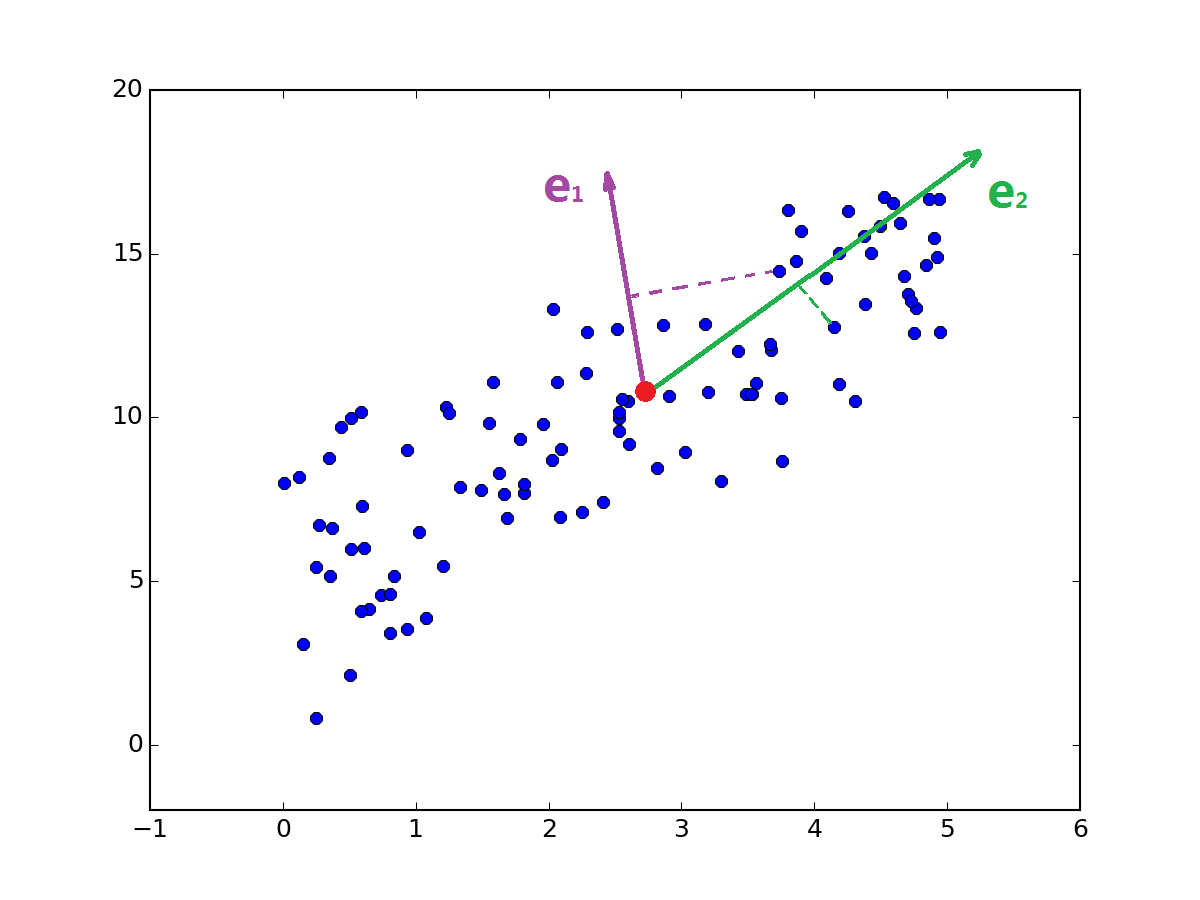
\includegraphics[width=0.5\textwidth]{trick/PCA_dot.eps}
\caption{二维空间中的数据样本点}
\label{img:PCA dot}
\end{figure}

如果我们通过计算得到这些样本点的均值$\bar{x}$,即
\begin{equation}
\bar{x} = \frac{1}{n}\sum\limits_{i=1}^n x^{(i)}
\end{equation}
正如图\ref{img:PCA dot}中的红点,那么我们总能将所有的点用一组基的线性组合来代替,即
\begin{equation}
x^{(i)} = \bar{x} + \alpha_1 e_1 + \alpha_2 e_2
\end{equation}
式中,$e_1$和$e_2$是任意两个不平行的单位向量,正如图\ref{img:PCA dot}中的紫色方向和绿色方向。但此时我们只是将样本点从一个原始的正交二维坐标系转换到另一个以$e_1$和$e_2$为基的二维坐标系,为了降维,我们必然需要舍弃一个维度,这个维度可能是$e_1$或$e_2$,然而选取哪个维度更好呢?直觉上我们会认为选取$e_2$会更好,因为当所有的数据点都投影到这个基上时,相比于$e_1$能更好地保留数据的信息。

然而,$e_1$和$e_2$是我们任意选取的两个基向量,事实上有可能有另外的基向量要比$e_1$更好的保留原始数据的特征,假设最优的基向量为$e$,那么为了刻画数据降维后原始数据与降维后数据的差异性,我们引入一个准则函数
\begin{equation}
J(\alpha_1, \alpha_2, \cdots, \alpha_n) = \sum\limits_{i=1}^n \bigg((\bar{x}+\alpha_i e) - x^{(i)}\bigg)\bigg((\bar{x}+\alpha_i e) - x^{(i)}\bigg)^T
\label{equ:PCA J}
\end{equation}
式中,$\bar{x}+\alpha_i e$实质上代表的是原始数据降维到一维空间后在二维空间中的坐标,即原始数据在基向量$e$的投影点的二维坐标。准则函数使用的依然是我们非常熟悉的二范数,这个准则函数事实上刻画的是原始坐标到投影坐标距离的平方,也就是两者究竟相差了多远。为了最小化这个准则函数,我们先对式\eqref{equ:PCA J}进行展开,这将得到
\begin{equation}
J(\alpha_1, \alpha_2, \cdots, \alpha_n, e) = \sum\limits_{i=1}^n \alpha_i^2 ||e||^2 - 2\sum\limits_{i=1}^n \alpha_i e^T(x_i - \bar{x}) + \sum\limits_{i=1}^n ||x_i - \bar{x}||^2
\end{equation}
由于$\sum_{i=1}^n ||x_i - \bar{x}||^2$只与数据相关而与参数无关可以舍去,此外,$e$是单位向量,所以$||e||^2$等于1,因此准则函数可以简写为
\begin{equation}
J(\alpha_1, \alpha_2, \cdots, \alpha_n, e) = \sum\limits_{i=1}^n \alpha_i^2  - 2\sum\limits_{i=1}^n \alpha_i e^T(x_i - \bar{x})
\label{equ:8.yyyy}
\end{equation}
为了最小化这个准则函数,我们对其求偏导,并另导数为0,则
\begin{equation}
\frac{\partial}{\partial \alpha_i} = 2\alpha_i - 2e^T(x_i - \bar{x}) = 0
\label{equ:8.xxxxxxx}
\end{equation}
因此当$\alpha_i = e^T(x_i - \hat{x})$准则函数取得最小。这实质上说明,当数据点投影到$e$时使得准则函数最小,与我们前面的猜测符合。将\eqref{equ:8.xxxxxxx}代回\eqref{equ:8.yyyy},我们便可以消去准则函数中的$n$个变量$\alpha_1, \cdots, \alpha_n$,只剩余一个变量$e$,即
\begin{equation}
J(e) = - \sum\limits_{i=1}^n e^T(x_i - \hat{x})(x_i - \hat{x})^Te
\end{equation}
如果我们记号散布矩阵为
\begin{equation}
S =\sum\limits_{i=1}^n (x_i - \hat{x})(x_i - \hat{x})^T
\end{equation}
则准则函数可以谢伟
\begin{equation}
J(e) =  -  e^TSe
\end{equation}
此时是一个约束优化问题,约束条件为等式约束$e^Te = 1$,为此引入拉格朗日乘子$\lambda$,构造拉格朗日函数为
\begin{equation}
\mathcal{L}(e) = - e^TSe + \lambda(e^Te-1)
\end{equation}
对拉格朗日求偏导,并另偏导为0
\begin{equation}
\frac{\partial}{\partial e} \mathcal{L}(e) = -2Se + 2\lambda e = 0
\end{equation}
此时说明,当$Se = \lambda e$时,准则函数最小,而事实上这是矩阵对特征根的定义,因此为了最小化准则函数,基向量$e$应当选取为散布矩阵$S$的特征向量。这个结论可以很容易推广到高维情况,假设我们有n个d维的数据样本,那么我们总能构造他的散布矩阵$S$,为了将它降到$k$维而同时又要使得准则函数最小化,我们应该选取$S$最大的$k$个特征值所对应的特征向量作为投影基,从而新的$k$维坐标为
\begin{equation}
\alpha_i = e^T(x^{(i)} - \hat{x})
\end{equation}

由于特征向量之间是正交的,因此降维后的数据在各个维度是独立的,这也是白化的目的,因此主成分分析也是一种白化方法。有时候我们需要将降维后的数据还原回原始的维度以检测降维后的数据究竟损失了所烧信息,那么利用特征向量的正交性,有
\begin{equation}
e\alpha_i = ee^T(x^{(i)} - \hat{x}) = x^{(i)} - \hat{x}
\end{equation}
此时等号两边同时加上均值$\hat{x}$即可还原出$d$维数据。如图\ref{img:PCA reconstruct}所示是$28\times 28$像素的图像,它共有784维,其原始数据为黑底的图像所示。如果我们使用主成分分析将其降到20维后再将其还原成784维数据,其图像如灰底图像所示,我们可以看到,经过降维后再还原的数据已经变得模糊化,而这些模糊化并不会影响我们对数字的识别。

\begin{figure}[!htbp]
\centering
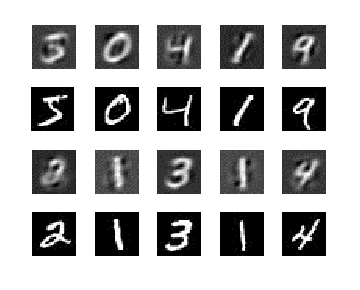
\includegraphics[width=0.3\textwidth]{trick/PCA.eps}
\caption{经过主成分分析降维后还原的数据}
\label{img:PCA reconstruct}
\end{figure}


\BiSubsubsection{多维尺度分析}
x在介绍多维尺度分析\citeup{kruskal1964multidimensional}之前,我们先从地图重构的问题讲起。假设我们在中国地图中选取五个城市,分别为北京、上海、广州、兰州、哈尔滨,依次用A、B、C、D、E代替。如果我们以北京为坐标平面的原点,那么剩下的城市坐标分别为:上海$(631.6, -796.4)$、广州$(103.8, -2029.2)$、兰州$(-1228, -428.1)$、哈尔滨$(265, 1082)$,将这些城市的坐标描绘在平面直角坐标系上的结果如图\ref{img:city map}所示。另外,我们可以通过计算得到这五个城市的两两距离如图\ref{img:city distance}所示。
\begin{figure}[htbp]
\centering
\subfigure{\label{img:city map}}\addtocounter{subfigure}{-2}
\subfigure{\subfigure[城市分布图]
			{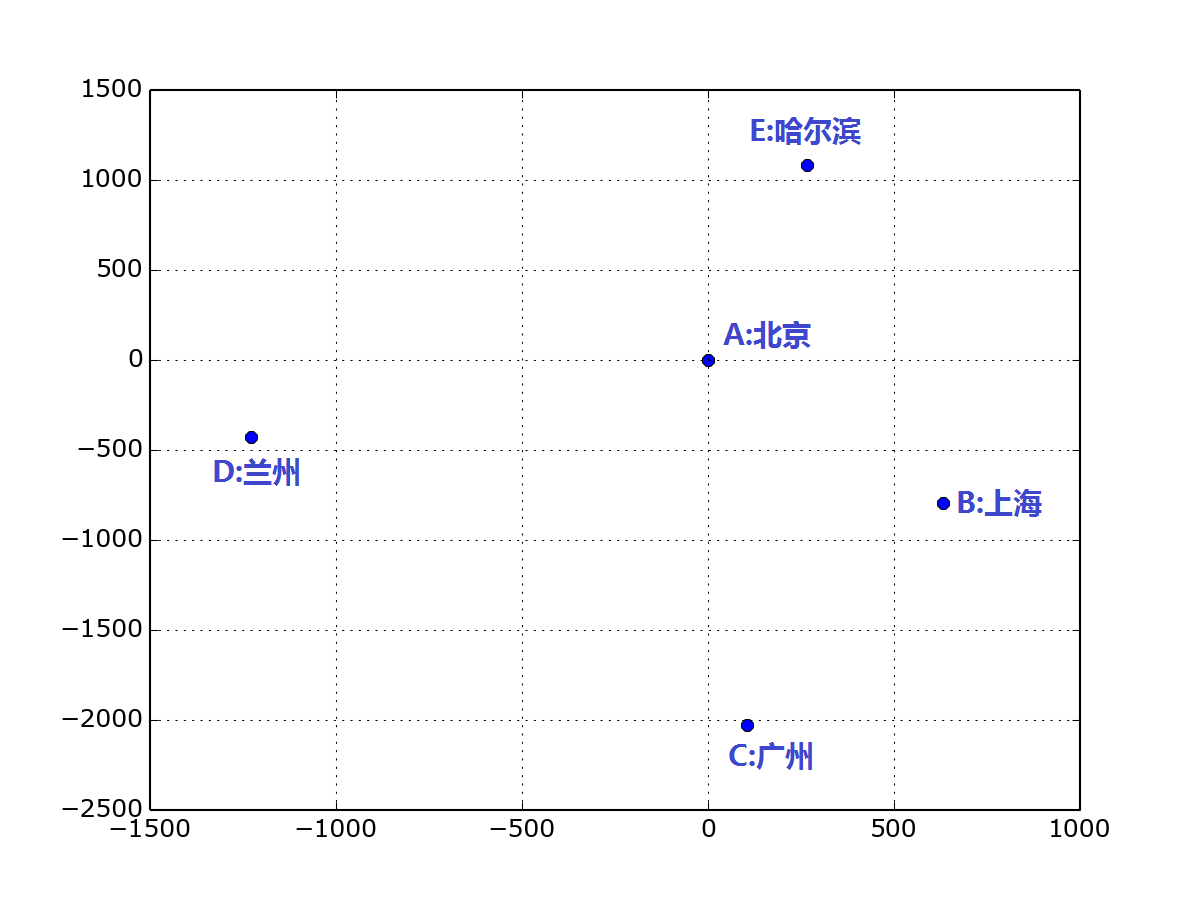
\includegraphics[width=0.48\textwidth]{trick/map_pure.eps}}}
\subfigure{\label{img:city distance}}\addtocounter{subfigure}{-2}
\subfigure{\subfigure[城市间两两距离]
			{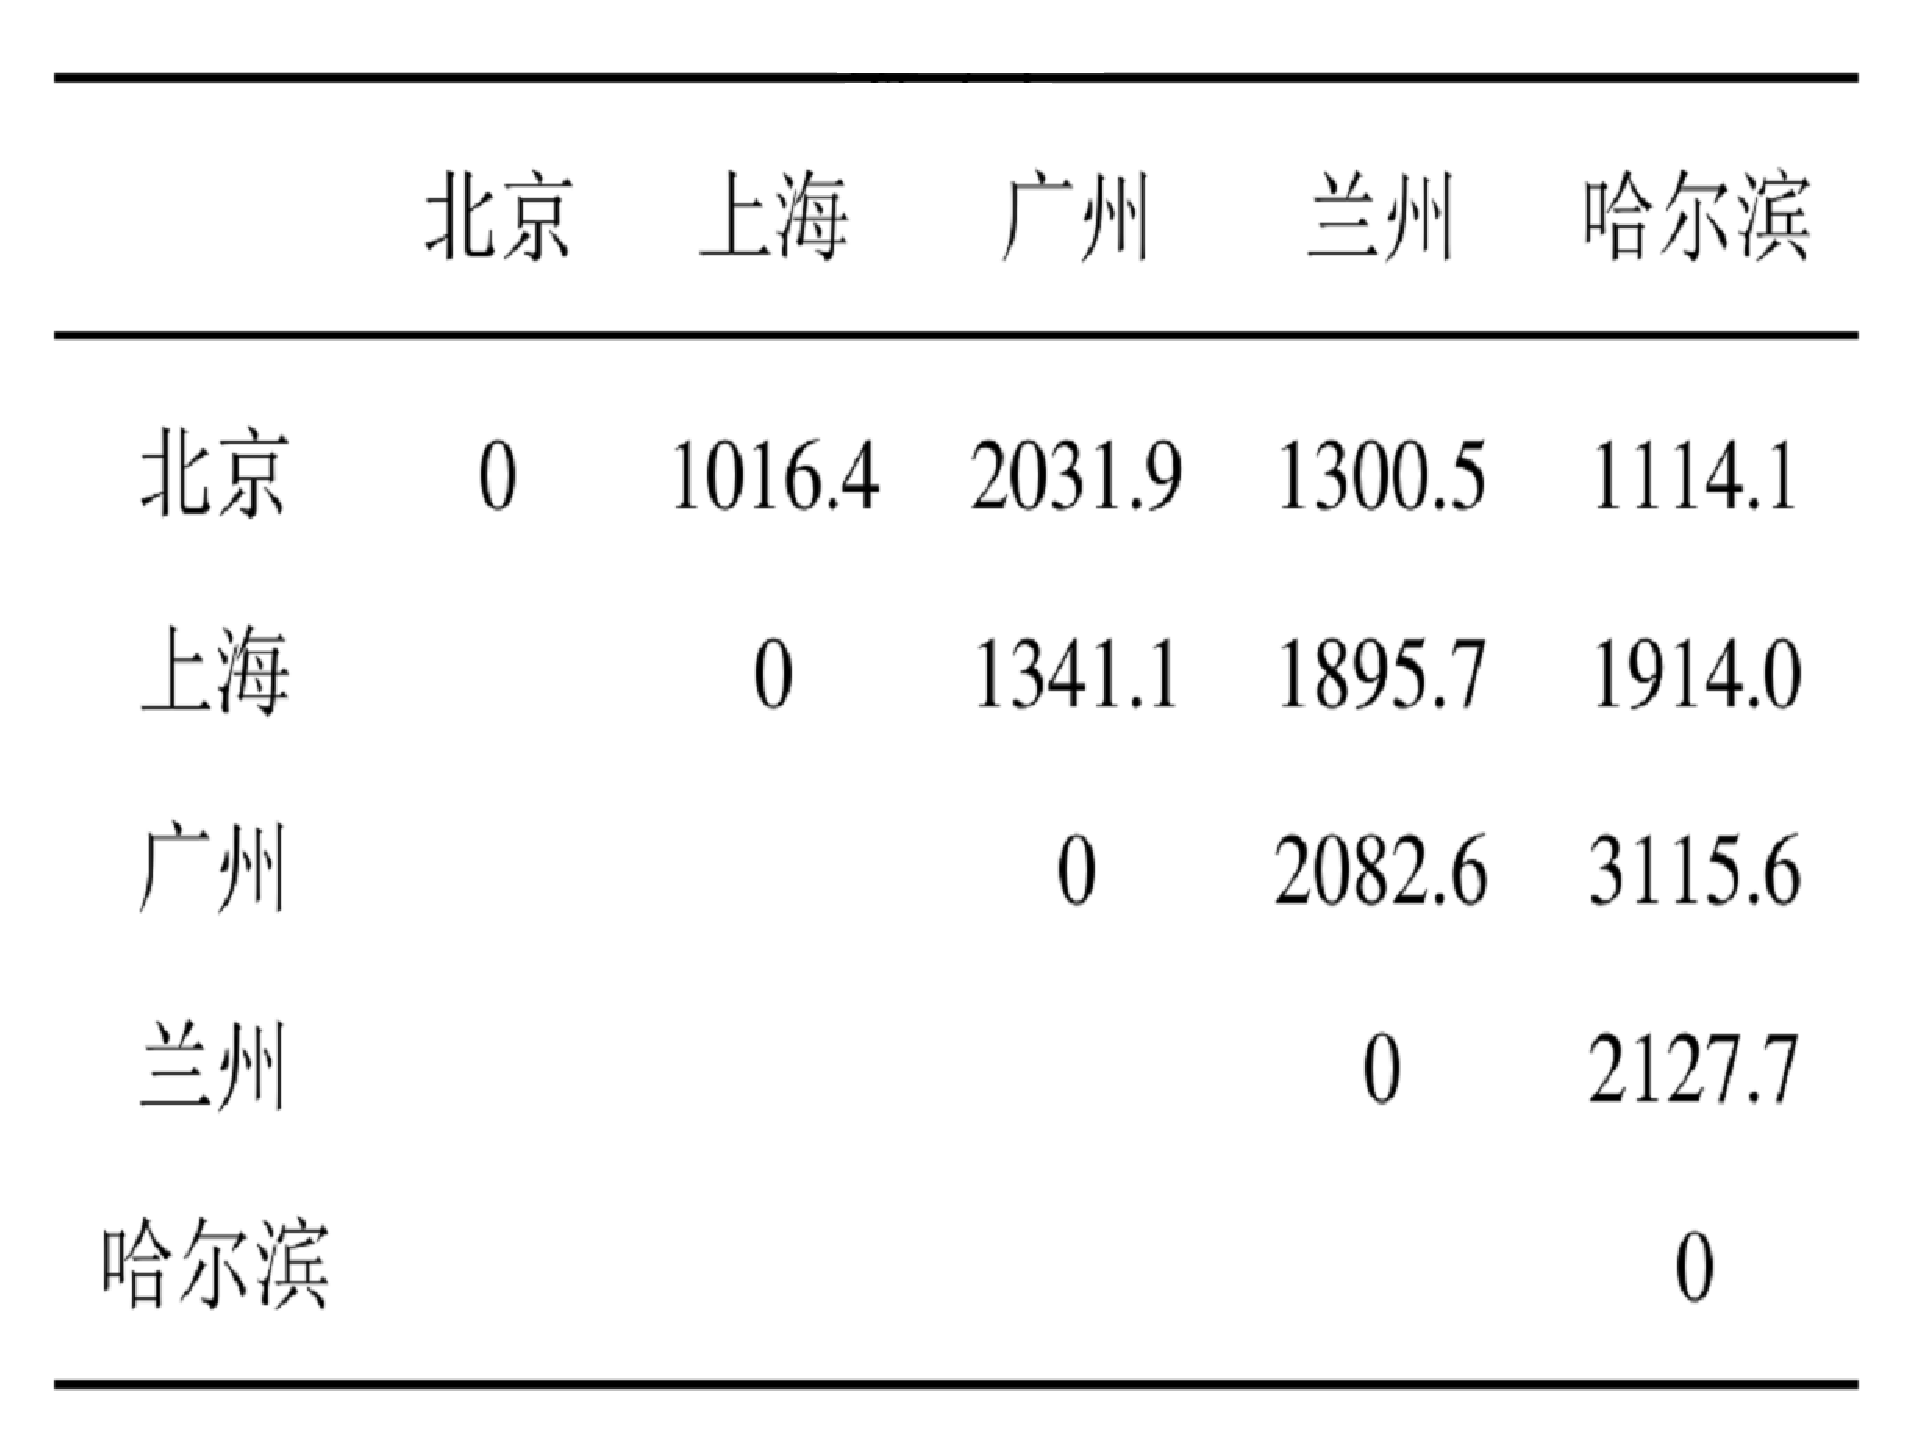
\includegraphics[width=0.45\textwidth]{trick/map_dist.eps}}}
\caption{五个城市的信息}
\vspace{-1em}
\end{figure}

如果现在我们不再知道各个城市的具体坐标,我们只知道图\ref{img:city distance}中两两城市之间的距离,那么如何通过图\ref{img:city distance}中的信息进行地图的重建,或者说根据距离推导出各个城市的坐标呢?这就是多维尺度分析所要完成的工作。

首先,我们假设这$n$个城市的坐标构成一个矩阵$X = [x_1, x_2, \cdots , x_n]^T$,那么城市$i$和城市$j$之间的欧式距离的平方为
\begin{equation}
s_{ij} = (x_i - x_j)^T (x_i, x_j)
\end{equation}
由$s_{ij}$可以构成一个$n\times n$的矩阵$S_{n\times n}$,这个矩阵我们称为距离矩阵,如果我们再定义Gram矩阵为
\begin{equation}
G_{n\times n} = HXX^TH
\end{equation}
其中,$H$为去中心化矩阵,定义为
\begin{equation}
H = I_n - ee^T
\end{equation}
其中,$I_n$为$n$阶单位矩阵,$e = \frac{1}{\sqrt{n}}(1, \cdots, 1)^T$,那么Gram矩阵可以推导为
\begin{equation}
G_{n\times n} = HXX^TH = \bigg[(x - \bar{x})^T (x - \bar{x})\bigg]
\label{equ:gram matrix}
\end{equation}
式中,$\bar{x}$为$X$的均值,通过式\eqref{equ:gram matrix},进一步可以推导得
\begin{equation}
G_{n\times n} = -\frac{1}{2}HSH
\end{equation}
由于欧几里得距离是正定的,因此Gram矩阵也是正定的,如果我们将Gram矩阵特征分解,则有
\begin{equation}
G_{n\times n} = P\Sigma P^T
\end{equation}
式中,$\Sigma$为Gram矩阵特征值构成的对角矩阵
\begin{equation}
\Sigma = \left[
\begin{array}{ccc}
\lambda_1 & &\\
&\ddots&\\
&&\lambda_n
\end{array}
\right]
\end{equation}
$P$为Gram的特征向量构成的矩阵,即$P = [p_1, \cdots, p_n]$。如果我们提取出Gram矩阵最大的k个特征值以及其对应的特征向量,那么通过
\begin{equation}
\hat{X} = \left[
\begin{array}{ccc}
\sqrt{\lambda_1} & &\\
&\ddots&\\
&&\sqrt{\lambda_k}
\end{array}
\right] 
[p_1, \cdots, p_k]
\end{equation}
我们将得到含有$n$个$k$维向量的矩阵$\hat{X}$,这个矩阵$\hat{X}$就是$X$在$k$维空间的一个映射。例如,在我们地图重构的问题中,通过图\ref{img:city distance}中的距离信息,当$k=2$时,我们求得
\begin{equation}
\hat{X} = \left[
\begin{array}{cc}
-45.6 & 434 \\
-677.1 & -362.1 \\
-149.3 & -1594.9 \\
1182.5 & 6.2 \\
-310.5 &1516.5
\end{array}
\right]
\end{equation}

如果将上述求得的坐标描绘在平面直角坐标系上,其结果如图\ref{img:map_mds_not_rot}所示。我们可以看到,这些点与真实分布十分相似,只相差一个水平镜像,我们将其镜像后的结果如图\ref{img:map_mds_rot}所示。镜像结果显示,重构的地图中,各个城市所在的相对位置与真实地图中城市的相对位置相同,但是不同的是,在重构的地图中,绝对位置改变了,例如我们可以看到,原来处于原点位置的北京现在不在处于原点。

\begin{figure}[htbp]
\centering
\subfigure{\label{img:map_mds_not_rot}}\addtocounter{subfigure}{-2}
\subfigure{\subfigure[重构后得到的直接结果]
			{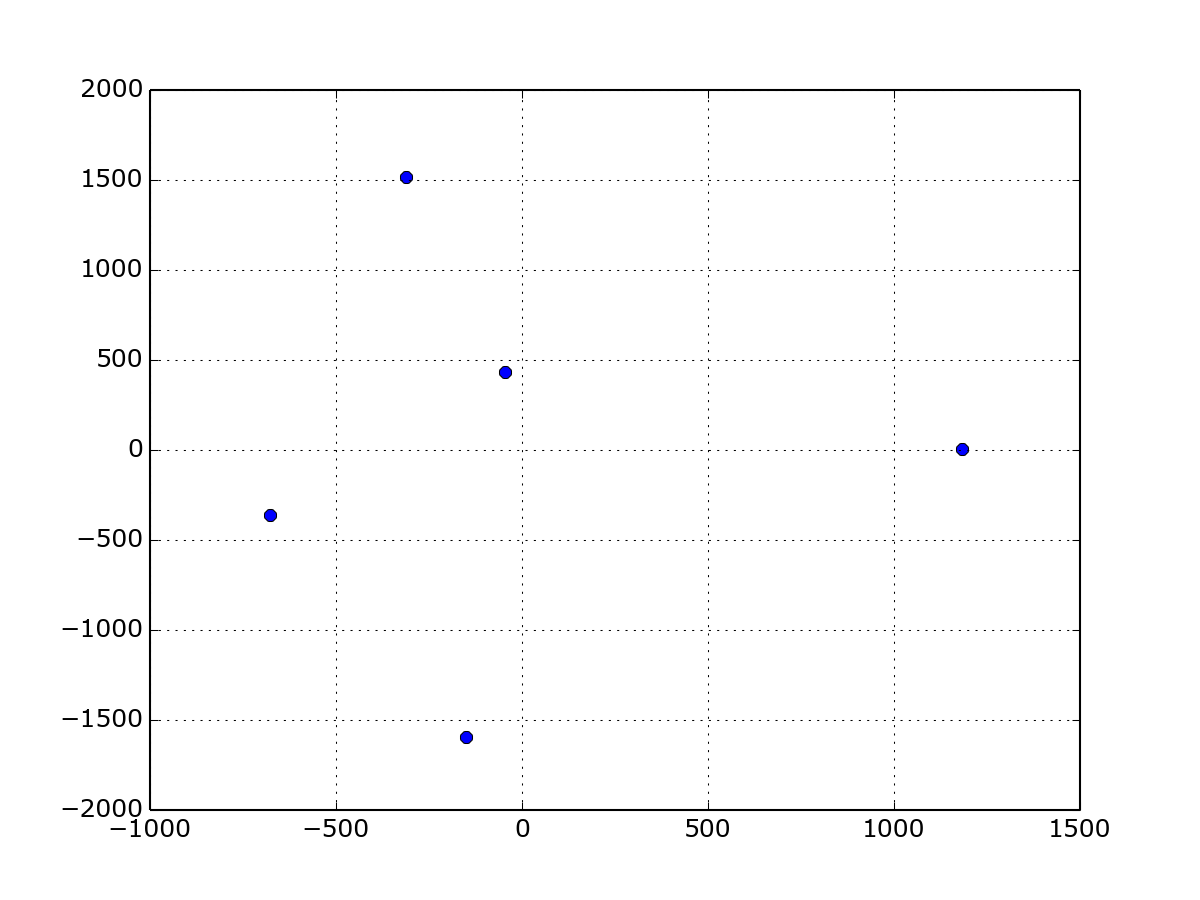
\includegraphics[width=0.45\textwidth]{trick/map_mds_not_rot.eps}}}
\subfigure{\label{img:map_mds_rot}}\addtocounter{subfigure}{-2}
\subfigure{\subfigure[镜像后的结果]
			{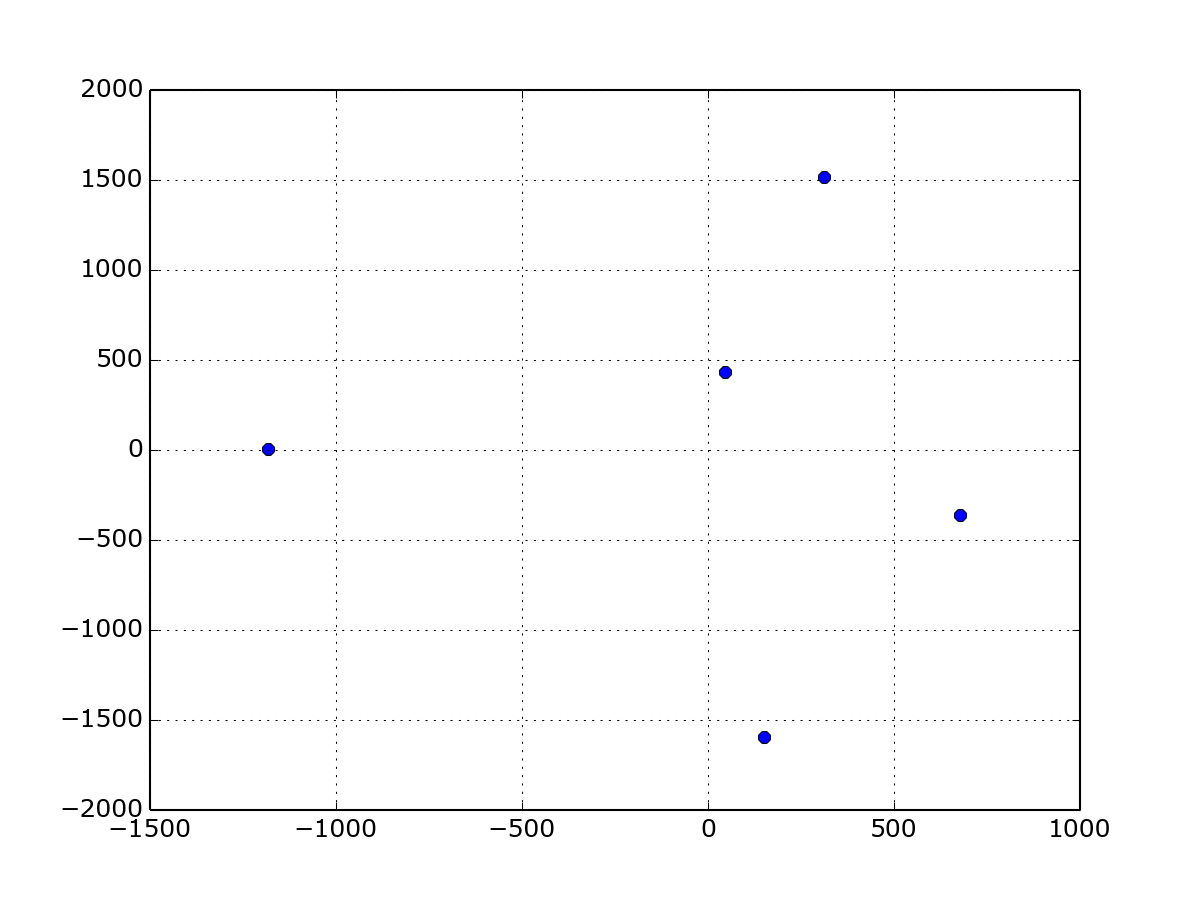
\includegraphics[width=0.45\textwidth]{trick/map_mds_rot.eps}}}
\caption{多维尺度分析对地图的重构}
\vspace{-1em}
\end{figure}

地图重构的例子并没有展现出多维尺度分析是如何降维的,因为这里只是从一个二维坐标转换到另一个二维坐标。但由于这个转换的过程中使用的欧几里得距离对于高维空间是可复用的,因此对于多维尺度分析的降维,我们先通过高维空间中的数据点两两求距离,得到平方距离矩阵,在通过这个平方距离矩阵求取Gram矩阵,将Gram矩阵特征分解,选取最大的$k$个特征值以及对应的特征向量,利用他们可以将原始的高维数据降到$k$维数据。例如,图\ref{img:MDS dim redu}描述了三维空间中的数据降到二维空间的过程。

\begin{figure}[htbp]
\centering
\subfigure{}\addtocounter{subfigure}{-2}
\subfigure{\subfigure[三维空间中的原始数据]
			{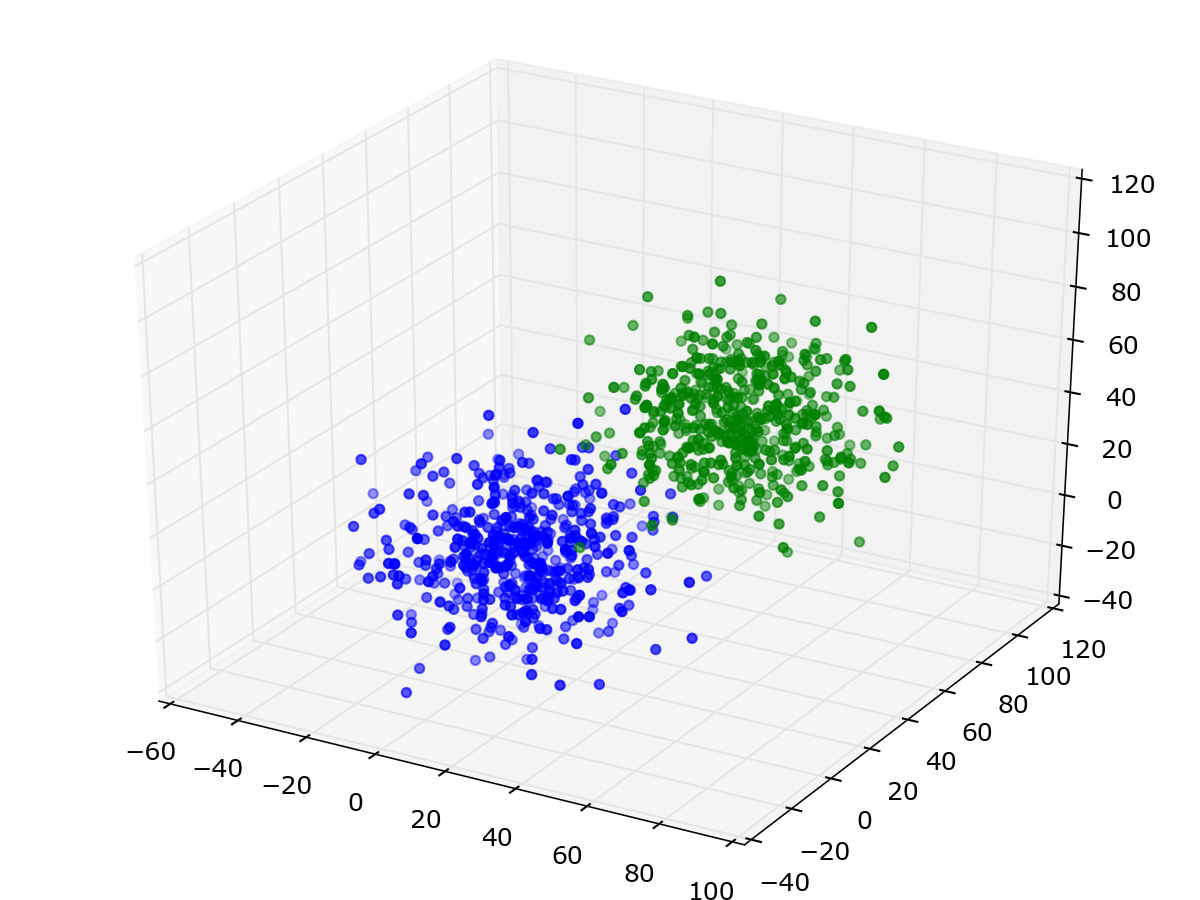
\includegraphics[width=0.45\textwidth]{trick/mds3D.eps}}}
\subfigure{}\addtocounter{subfigure}{-2}
\subfigure{\subfigure[降到二维空间后的数据]
			{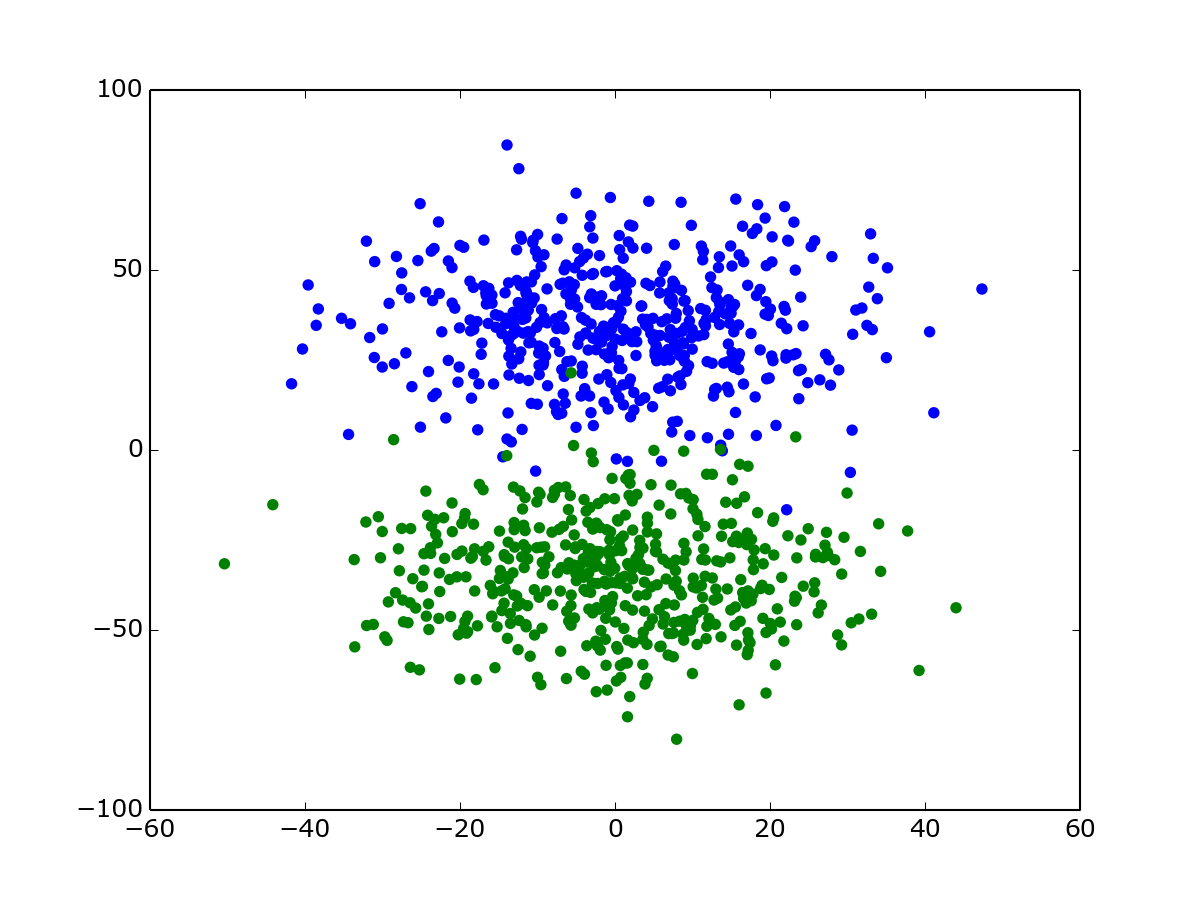
\includegraphics[width=0.45\textwidth]{trick/mds2D.eps}}}
\caption{多维尺度分析的降维}
\label{img:MDS dim redu}
\vspace{-1em}
\end{figure}

多维尺度分析并不是一个应用非常广泛的降维方法,其主要原因在于欧几里得距离,如图\ref{img:swiss roll 2}三维空间中AB两点,如果使用欧几里得距离(图中的绿线),那么我们认为这两点是十分接近的,因此降到二维空间后这两点将会靠得很近。但事实上AB两点相距很远,它们两者之间经过很长一段流形(图中的红线),而欧几里得距离忽视了这种距离。

\begin{figure}[!htbp]
\centering
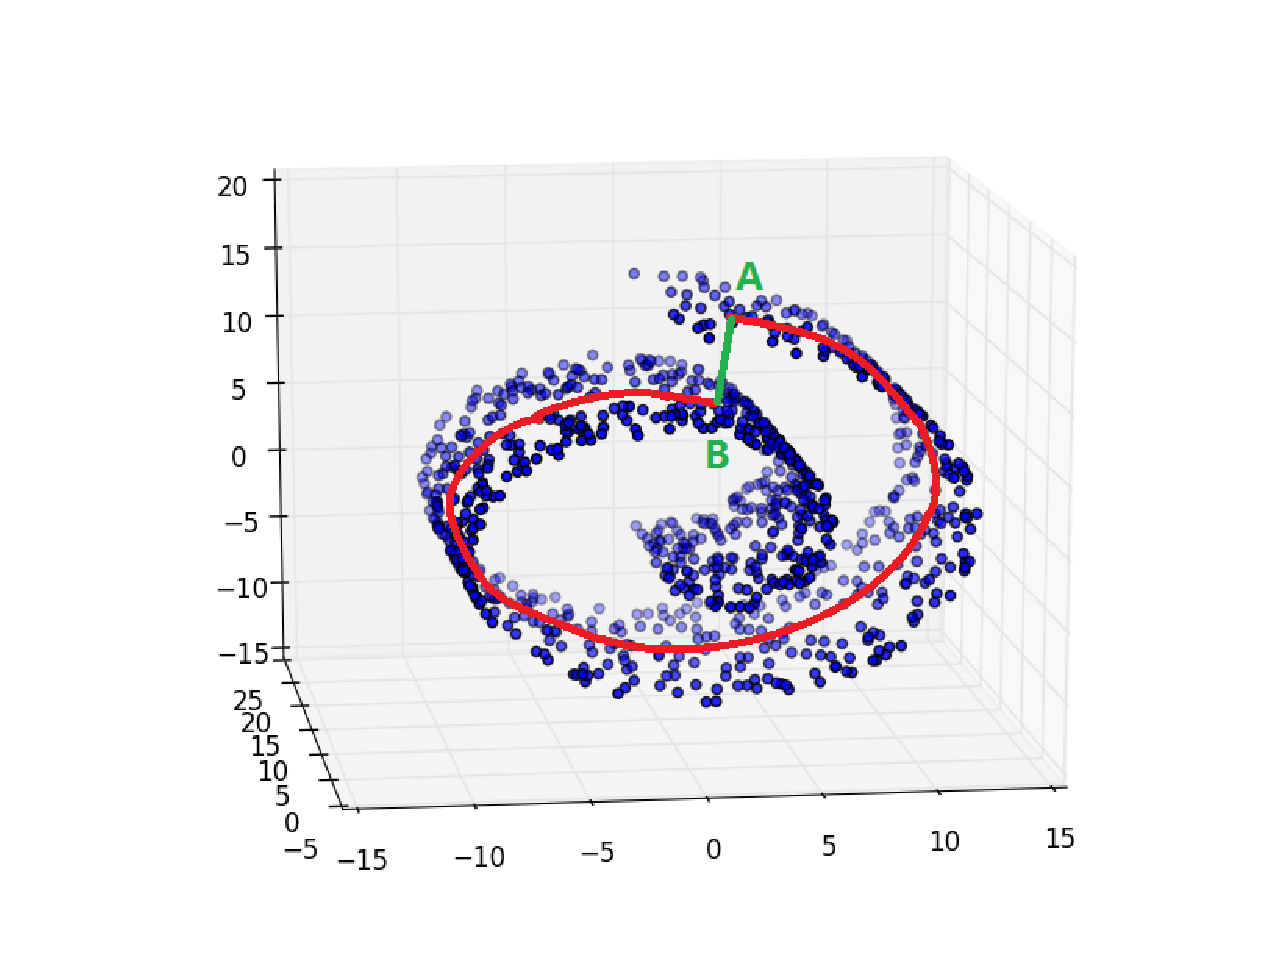
\includegraphics[width=0.8\textwidth]{trick/swissRoll2.eps}
\caption{Swiss Roll}
\label{img:swiss roll 2}
\end{figure}

尽管多维尺度分析并不常用,但是通过它可以引入流形学习中的一些经典算法,例如Isomap等,用以解决图\ref{img:swiss roll 2}中类似的情况,更多的讨论可参考文献xxxx

\BiSubsection{扩容}
x机器学习业内有一个共识,很多时候别人的分类性能比你的好并不意味着他的算法比你的好,更大的可能是他拥有比你更多的数据。数据是统计机器学习的命脉,没有数据,再好的模型也难以奏效。如果把机器学习中的算法比作是航天器的引擎,那么数据就是航天器的燃料。这种现象在深度学习中尤为明显,特别是卷积神经网络。深度学习需要大量的数据样本,这个需求量随着识别任务复杂性的增加而增加。尽管互联网的大数据时代数据容易获取,但有些时候数据是有限的,对于有限的数据集,我们可以通过一定的手段将数据集的容量扩大。例如在字符识别任务中,我们知道,字符微量的扭曲、旋转、放大、缩小对人而言是不会影响字符的识别,因此,我们可以对原始数据进行随机地选取上述一个或多个变换,使得数据的容量增大。又例如,真实生活中的图片,水平镜像、对比度微调、饱和度微调等操作对人而言不影响最终的图像识别,我们利用这个特性对图像采取一定的变换便可很大程度地增大训练集的容量,例如,仅仅是图像的水平镜像就可以使得数据集扩大一倍。

数据的扩容,实质上是一种贝叶斯先验,因为我们对数据采取的变换策略不会影响最终的分类,例如,我们不会对字符进行镜像处理。这种先验,使得模型可以免疫一定的干扰,例如采取了水平位移变换策略的数据集受到水平位移的影响就减小了,这就提高了模型的泛化能力。

\BiSection{训练技巧}
x网络的训练过程中,我们会使用到一些技巧,这些技巧大部分的目的都在于抑制网络的过拟合以及防止准则函数陷入局部最优解。由于这些技巧众多,我们无法在这里涵盖所有,因此我们只挑选了几个常用且重要的技巧,分别是学习率的设定、动量项的使用以及权衰减。
\BiSubsection{学习率}
x在梯度下降算法中,每次求得准则函数相对于参数的梯度$\partial J /\partial \theta$后,我们并不是直接以这个值作为参数的增量,工程中,我们还应对梯度乘上一个学习率$\eta$,即参数更新的公式为
\begin{equation}
\theta = \theta - \eta \frac{\partial J}{\partial \theta}
\label{equ:grandianDes}
\end{equation}
学习率的作用类似于下山时步伐的长度,步伐过长,则有可能导致准则函数震荡,影响收敛速度,如果步伐十分大,则会导致发散现象,哪怕准则函数是凸函数,存在唯一极值点,过大的学习率也会使其发散。例如,假设准则函数设定为二次函数,即
\begin{equation}
J(\theta) = \theta^2
\end{equation}
显然这是一个凸函数,存在唯一极值点,即$\theta = 0$处。如果我们对这个准则函数求偏导,则为
\begin{equation}
\frac{\partial J}{\partial \theta} = 2\theta
\end{equation}
即准则函数$J(\theta)$上的每一点$\theta$,其梯度都等于$2\theta$。假设现在$\theta = 2$,那么我们可以很容易计算得到其梯度为$4$,此时,最优的学习率为$\eta ^* = 0.5$,因为$2-0.5\times 4$恰好使得$\theta$落入到最优解即$\theta = 0$处,如图\ref{img:eta=0.5}所示。如果我们的学习率选取得比最优学习率大,假设我们选取为$\eta  = 0.7$,那么参数$\theta$就会沿着$2\rightarrow \rightarrow -0.8\rightarrow 0.32 \rightarrow -0.128 \cdots$的轨迹下降,如图\ref{img:eta=0.7}所示。倘若我们的学习率再大一些,为两倍的$\eta$时,即当$\eta  = 1$时,$\theta$就会在$+2$和$-2$两者之间变换而不会进入别的位置,如图\ref{img:eta=1}所示。当学习率大于两倍的最优学习率,例如$\eta = 1.5$,那么$\theta$就会沿着$2\rightarrow -4 \rightarrow 8\rightarrow -16$的轨迹移动,此时准则函数便发散,这个过程如图\ref{img:eta=1.5}所示。

\begin{figure}[htbp]
\centering
\subfigure{\label{img:eta=0.5}}\addtocounter{subfigure}{-2}
\subfigure{\subfigure[$\eta = 0.5$]
			{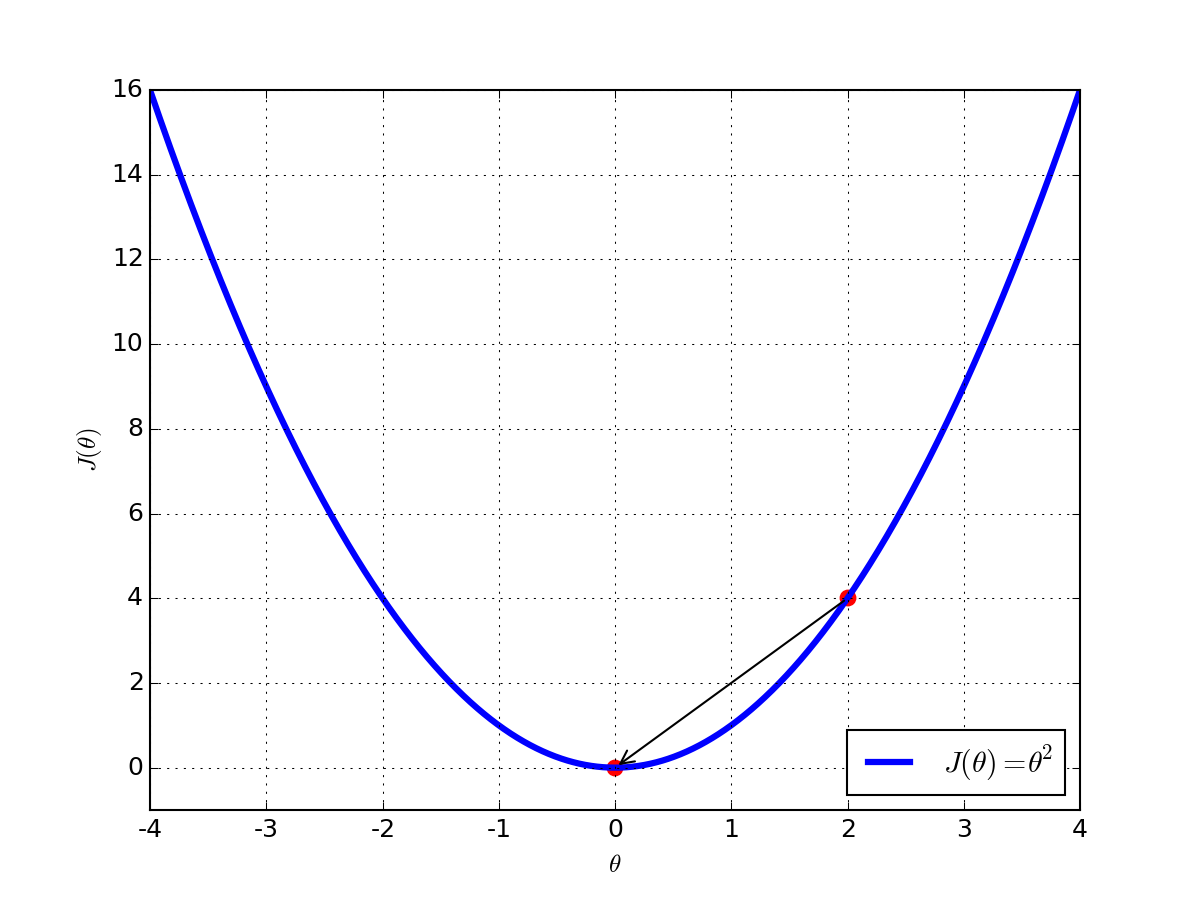
\includegraphics[width=0.4\textwidth]{trick/eta05.eps}}}
\subfigure{\label{img:eta=0.7}}\addtocounter{subfigure}{-2}
\subfigure{\subfigure[$\eta  = 0.7$]
			{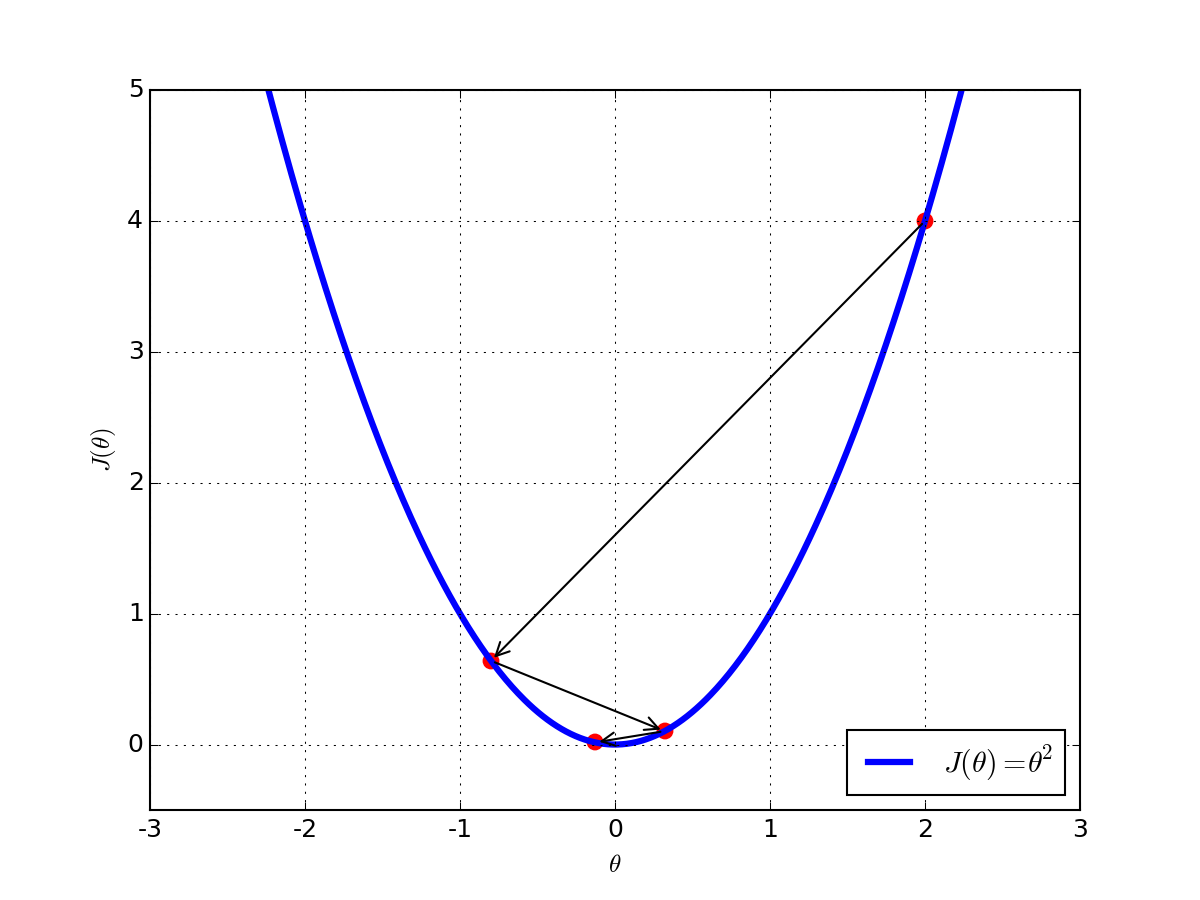
\includegraphics[width=0.4\textwidth]{trick/eta075.eps}}}
\subfigure{\label{img:eta=1}}\addtocounter{subfigure}{-2}
\subfigure{\subfigure[$\eta  = 1$]
			{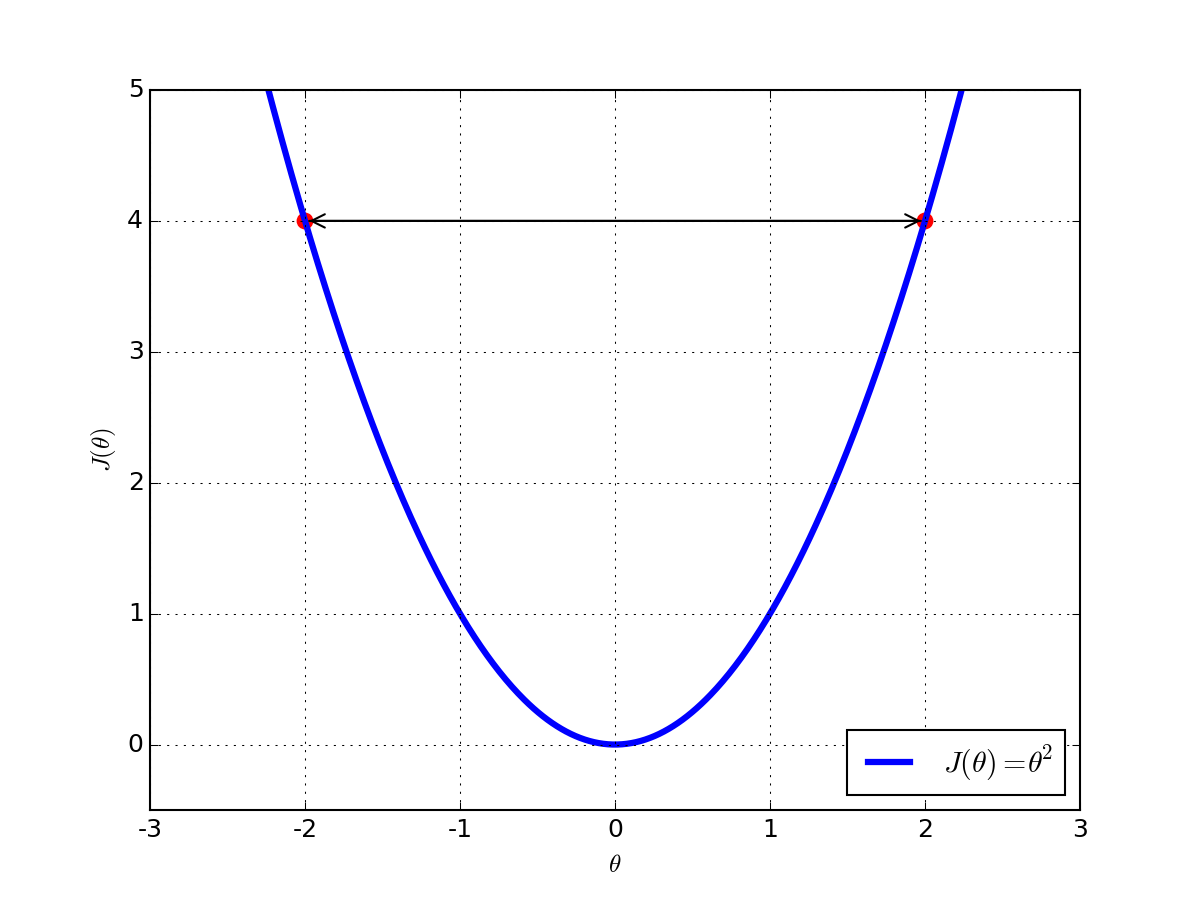
\includegraphics[width=0.4\textwidth]{trick/eta1.eps}}}
\subfigure{\label{img:eta=1.5}}\addtocounter{subfigure}{-2}
\subfigure{\subfigure[$\eta = 1.5$]
			{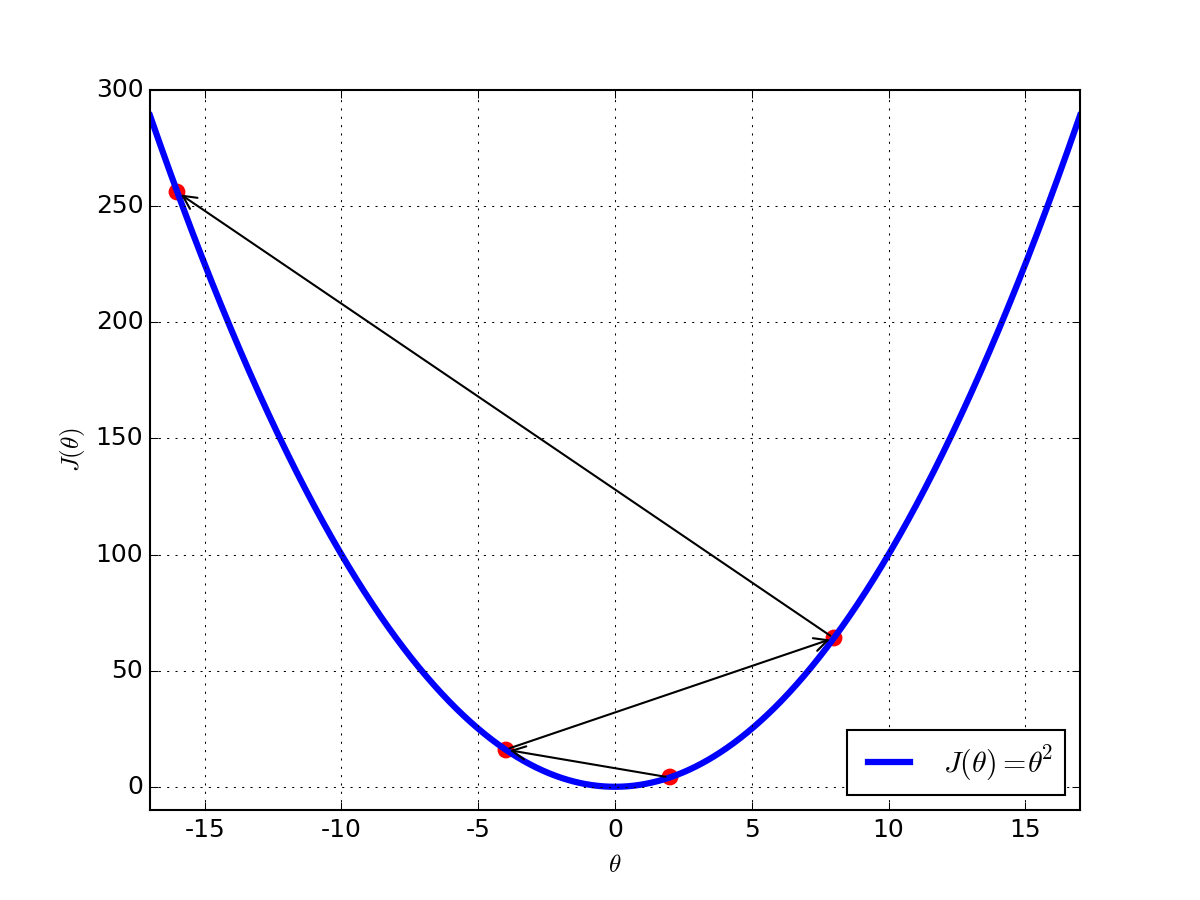
\includegraphics[width=0.4\textwidth]{trick/eta15.eps}}}
\caption{不同的学习率对收敛的影响}
\vspace{-1em}
\end{figure}


但是较大的学习率并不意味着一无是处,学习率稍微大一些,可以加快收敛速度,而且可以越过一些局部极小值(但是对于高尔夫球场形状的局部极小值无能为力)。在工程中,学习率的选取我们的建议是,先将学习率初始化为一个较大的数值,如果准则函数发散了,那么我们就将其缩小2倍,直到准侧函数能开始下降为止。另外一种做法是,先初步计算梯度的数值大小,将学习率设定为一个比梯度小3个数量级的常数,例如,我们上面的计算得到的梯度是4,那么学习率可以设定为0.001。

事实上学习率固定为一个常数并不是一个较好的策略,因为初始时设定的学习率相对于训练的后期而言是过大的,这将会导致准则函数在极小值附近震荡。一种解决方法是将学习率也设定为一个学习参数,这个参数随着网络的训练而不断地更新,另外一种虽然愚蠢但行之有效的方法是,不断地关注准则函数的下降情况,一旦感觉下降开始出现震荡或平谷现象就将学习率调小1个数量级。

\BiSubsection{动量项}
x很多时候,在参数校正的过程中,仅仅使用学习率是不行的,一般还应使用动量项。动量项,即在参数的更新过程中,引入一个动量因子,更新规则描述为
\begin{equation}
\theta_{t+1} = \theta_t - \eta(1-p)\frac{\partial J(\theta)}{ \partial \theta_t} - p * (\theta_{t-1} - \theta_{t-2})
\label{equ:momentum1}
\end{equation}
式中,$t$代表第$t$次参数更新,$\eta$为学习率,$p$为动量项因子,这个因子一般选取为$p = 0.9$。式\eqref{equ:momentum1}实际上讲述了这样一件事:参数更新的时候,增量不仅仅依赖于当前的梯度,还依赖于上一次权值变化量的$p$倍,因此参数的更新,带着类似于物理中动量的项,即$p * (\theta_{t-1} - \theta_{t-2})$,它也被称之为动量项。动量项可以使得准则函数快速地下降,并且可以越过一些较为平坦的局部极值。如果读者有数字信号处理的背景,式\eqref{equ:momentum1}实际上是一个脉冲响应低通滤波器,目的在于平滑参数的更新过程\citeup{Duda}。

但由于\eqref{equ:momentum1}需要记录上一次的参数增量,这在实际编码中需要一定的内存,而且实现起来也不方便,另外一种关于动量项的简单用法是
\begin{equation}
\theta_{t+1} = p\theta_t - \eta\frac{\partial J(\theta)}{ \partial \theta_t}
\end{equation}
式中,$p$为动量项系数,一般取0.9。动量项的使用,确实可以在一定程度上避免局部最优解,例如,假设准则函数为
\begin{equation}
J(\theta) = -5\theta^3 - 80\theta^2 - 400\theta - 700
\end{equation}
我们可以很容易地计算准则函数在任意一点的梯度为
\begin{equation}
\frac{\partial J(\theta)}{ \partial \theta} = -15\theta^2 - 160\theta - 400
\end{equation}
假设学习率设置为常数0.001,如果不采用动量项,即参数更新的规律为
\begin{equation}
\theta =\theta - 0.001\frac{\partial J(\theta)}{ \partial \theta} 
\end{equation}
那么准则函数的收敛过程如图\ref{img:no momentum}所示,我们可以看到,在收敛的后半阶段,参数$\theta$会收敛到局部极值,但如果我们使用一个系数为0.9的动量项,即参数更新规则为
\begin{equation}
\theta =0.9 * \theta - 0.001\frac{\partial J(\theta)}{ \partial \theta} 
\end{equation}
此时的准则函数收敛过程如图\ref{img:has momentum}所示,我们可以看到,动量项的引入,使得参数$\theta$在平坦的局部极值区域内依然带有冲劲,这个性质使得它可以跨越一些较小的局部极值而不至于陷入其中。
\begin{figure}[htbp]
\centering
\subfigure{\label{img:no momentum}}\addtocounter{subfigure}{-2}
\subfigure{\subfigure[不使用动量项]
			{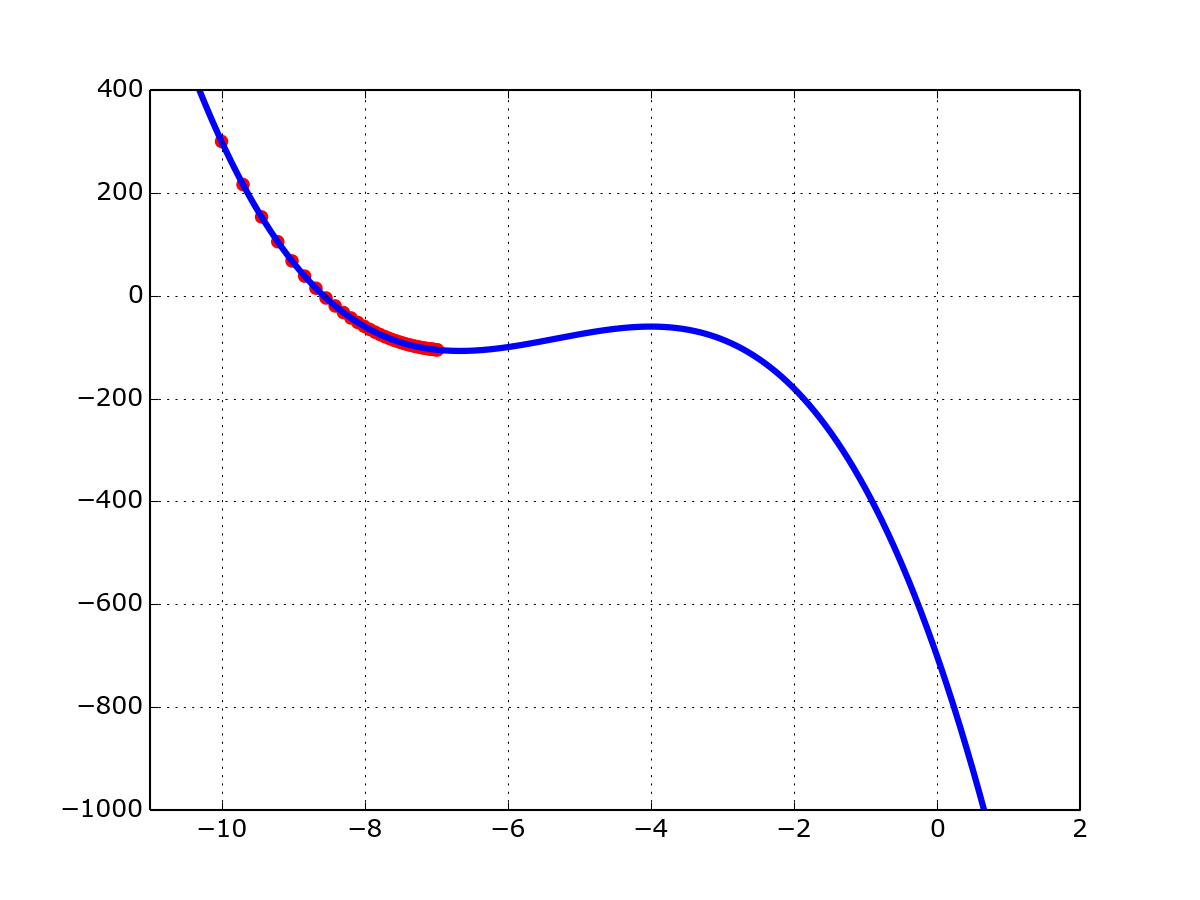
\includegraphics[width=0.45\textwidth]{trick/noMonent.eps}}}
\subfigure{\label{img:has momentum}}\addtocounter{subfigure}{-2}
\subfigure{\subfigure[使用系数为0.9的动量项]
			{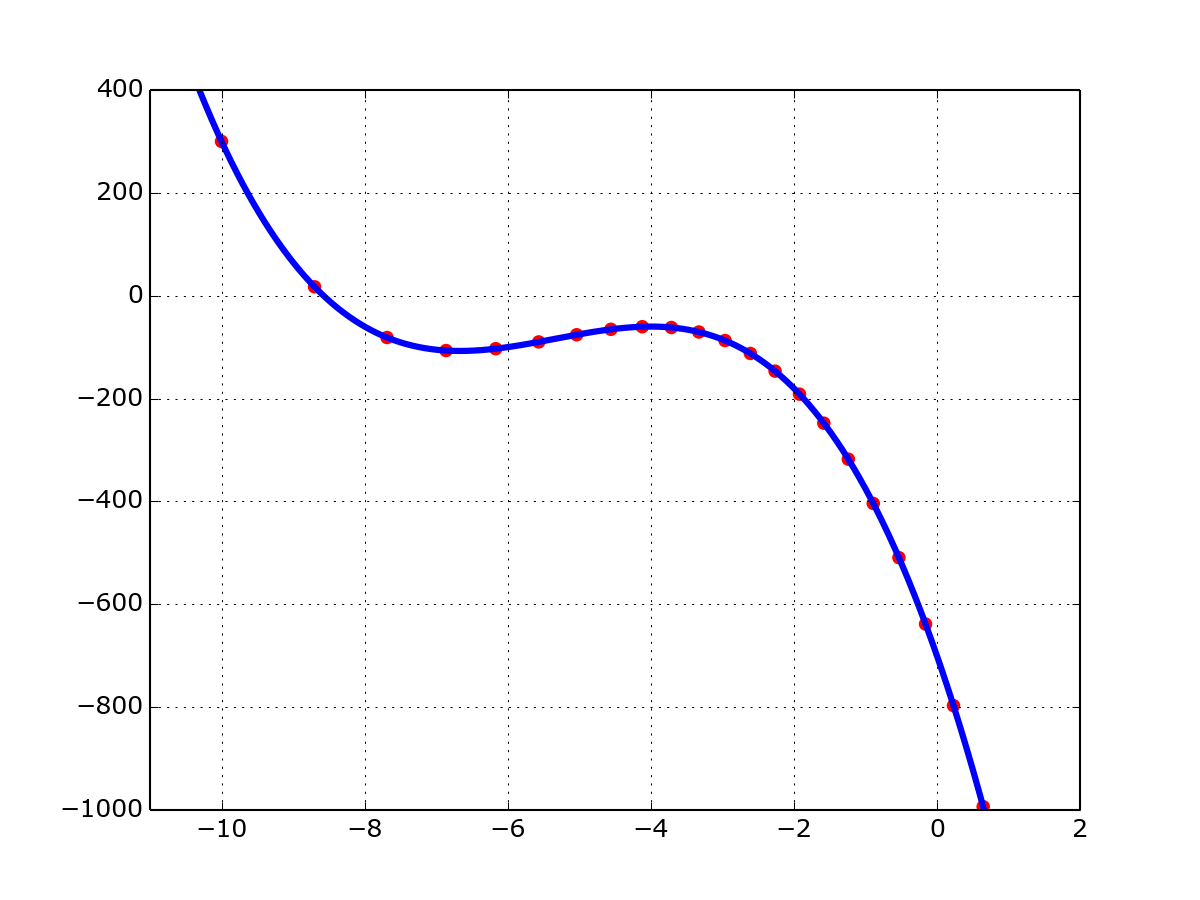
\includegraphics[width=0.45\textwidth]{trick/hasMonent.eps}}}
\caption{动量项对收敛的影响}
\vspace{-1em}
\end{figure}

\BiSubsection{权衰减}
所谓权衰减,即在权值更新完毕后对所有的权值乘以一个小于1的常数$e$,$e$一般取0.999左右。之所以要这样做的原因,是因为我们希望权值保持在较小的范围内,因为更小的权值使得净激活停留在激活函数的非饱和区域内。使用权衰减的参数更新规则为
\begin{equation}
\theta = e*\theta
\label{equ:weight decay}
\end{equation}
关于权衰减的另一种解释是,在准则函数中,我们加入一个二范数惩罚,即新的准则函数定义为
\begin{equation}
J_{new}(\theta) = J(\theta) + \frac{\lambda}{2} \theta^T\theta
\label{euq:penalyL2}
\end{equation}
\eqref{euq:penalyL2}中的第二项也被称为正则项。如果我们对式\eqref{euq:penalyL2}求导,则为
\begin{equation}
\frac{\partial J_{new}(\theta)}{ \partial \theta} = \frac{\partial J(\theta)}{ \partial \theta} + \lambda \theta
\end{equation}
因此权值的更新规则为
\begin{equation}
\theta = \theta - \frac{\partial J_{new}(\theta)}{ \partial \theta} = \bigg(\theta -  \frac{\partial J(\theta)}{ \partial \theta}\bigg) - \lambda \theta
\end{equation}

这事实上等价于是式\ref{equ:weight decay},即在权值更新后乘上一个衰减系数。我们之所以使用权衰减,或者说加入二范数正则(这两个命题等价),实际上它代表着一种贝叶斯先验,即我们对于权值的期待(希望它是较小的值)。

需要注意的是,在神经网络中,我们一般只针对权值进行权衰减,而不针对偏置进行权衰减,因为我们希望获得较大的偏置。至于为什么,这实际上并没有为什么。


\BiSection{编码技巧}
x尽管我们讨论了大量的理论内容,这些理论内容具体实现在代码上并不是一件简单的事。代码如何设计以及如何测试是我们遇到的最大问题。与传统的软件工程所不同的是,机器学习中的测试无法使用单元测试,因为在单元测试中我们需要知道代码的期望输出,机器学习自学习的特点注定了我们无法知道其正确输出是什么。代码的测试,更多时候是凭感觉,尽管如此,我们还是有办法进行一些简单测试的,在本小节中,我们将会介绍面向对象的设计思路以及用于测试的梯度校验。
\BiSubsection{面向对象技术}
x神经网络的设计中,不同层可以采用不同的激活函数,也可以采用不同的网络结构,例如卷积层或全连接层。这些不同层之间都有两个共同的特性。在前向传播过程中,无论是什么形式的层都接收前一层传播的激活,而在反向传播过程中,所有的层都接收后一层传播回来的误差,并利用该层的输入与输出对参数进行校正。尽管不同结构的网络层其校正方式不同,但这个过程可以使用面向对象的技术实现。为了方便讨论,我们将用JAVA的语法来描述这个过程\footnote{然而JAVA并不是一门适合数值运算的语言}。我们定义一个接口Layer,它含有两个方法,即fprop和bprop,分别对应着前向传播和反向传播。fprop接收一个参数,即前向传播得到的输入数据,bprop接收三个参数,分别是反向传播回来的误差、该层的输入以及该层的输出,事实上,bprop也可以设定为只接收一个参数,即反向传播回来的误差,而该层的输入以及该层的输出设定为成员变量。具体的网络结构,例如ConvlutionLayer、FullConnectLayer等实现这个接口,并实现这个接口中的两个方法,利用多态性,就可以容易地实现不同层执行不同的更新方法。如果网络的所有层都采用同一个激活函数,那么这个激活函数可以直接写到接口中(尽管JAVA要JDK9中才能在接口中提供方法的实现,但我们可以利用继承让具体的层继承另一个类)。如果网络的所有层采用的是不同的激活函数,那么我们可以通过策略模式将激活函数抽象成一个接口,具体的激活函数实现这个接口,在具体网络层实现类的构造方法中通过依赖注入将具体的激活函数实现注入到网络层的类中,利用多态性,可以让不同的层执行不同的激活函数,而这些不同的激活函数又可以实现代码复用。最后将这些不同的网络层组合到一个神经网络实现类中,例如CNN或DBN,即可完成整个网络的编码工作,整个工程代码的UML图如图\ref{img:UML}所示。
\begin{figure}[!htbp]
\centering
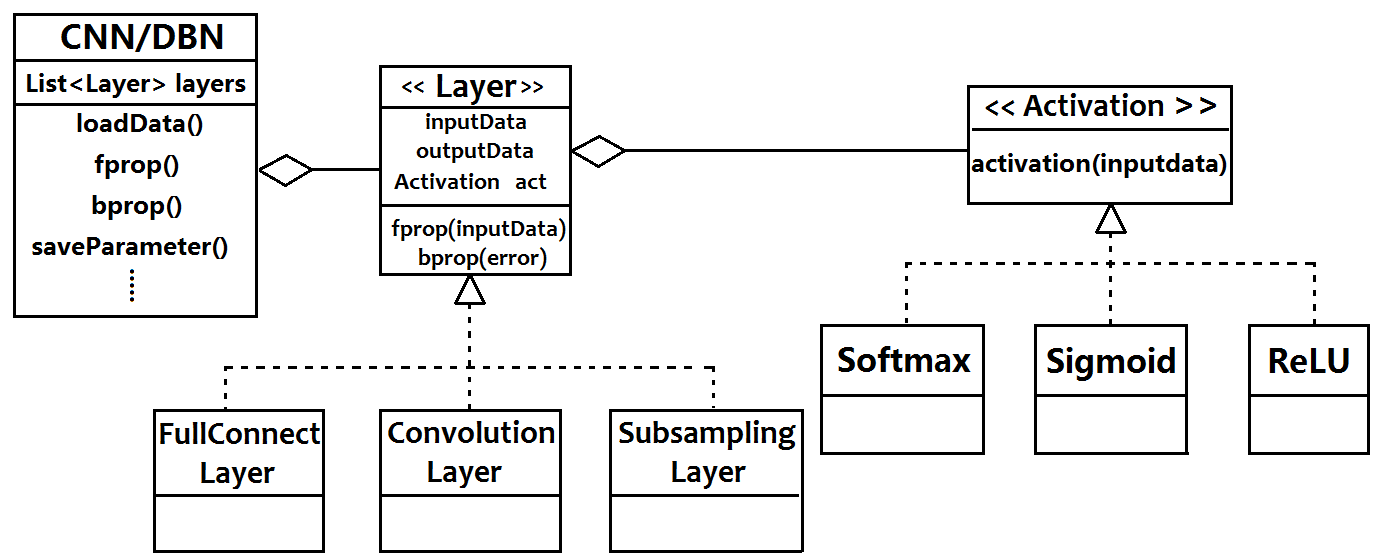
\includegraphics[width=1\textwidth]{trick/UML.eps}
\caption{神经网络类图设计}
\label{img:UML}
\end{figure}
\BiSubsection{梯度校验}
x在神经网络的编码中,一个令人头疼的问题是反向传播是否已经被正确编码。很多时候,错误的编码并不会导致严重的错误,但它会影响最终的分类效果。在debug过程中,一个十分有效的用来检测编码是否正确的方法是梯度校验。假设我们要优化以$\theta$为参数的准则函数,在梯度下降中,我们的更新规则如式\eqref{equ:grandianDes}所示。假设我们通过算法计算得到准则函数相对于参数的梯度,例如,在全连接神经网路中,这个梯度一般为
\begin{equation}
\frac{\partial J(\theta)}{\partial \theta} = \delta \cdot \frac{\partial f(net)}{\partial net} \frac{\partial net}{\theta}
\label{eqe:trickxxxx}
\end{equation}
式\eqref{eqe:trickxxxx}本质上是利用导数公式取计算梯度,正如我们要算$J(\theta) = \theta ^2$的导数,那么我们可以通过其导数即$J'= 2 \theta$直接计算在某点处的导数,但我们还可以通过另一种方式计算导数。回想高等数学中关于导数最原始的定义,导数即增量的极限,定义为
\begin{equation}
\frac{\partial J(\theta)}{\partial \theta} = \lim\limits_{\Delta\theta \rightarrow 0} \frac{J(\theta + \Delta\theta) - J(\theta)}{\Delta\theta}
\label{equ:limit}
\end{equation}
也就是说,如果我们给某个参数$\theta_i$加上一个非常小的增量$\Delta\theta$,假设为0.001,那么利用式\eqref{equ:limit}的原理,我们对比$\theta_i$没有加上这个增量之前准则$J(\theta)$的值与加上增量之后准则的值,这两个值作差,再除以增量,将会得到准则函数相对于$\theta_i$这个变量的梯度。这种方法求得的梯度$\Delta^*_\theta J(\theta)$与利用式\eqref{eqe:trickxxxx}$\Delta_\theta J(\theta)$满足如下关系
\begin{equation}
\Delta^*_\theta J(\theta) \approx \Delta_\theta J(\theta)
\end{equation}

如果$\Delta\theta$取得足够小,那么这两者近似程度非常高,但是实际编码中$\Delta\theta$不应取得过小,因为计算机的浮点运算会带来误差,一般而言,$\Delta\theta$取0.001左右就足以用来验证梯度了。另外需要注意的是,这种近似性只会在较深的层中发生,在较浅的层中误差会较大,因为反向传播是贪婪的,所以随着误差越传越远,梯度的偏离也会越大。利用梯度校验在可以方便检验代码正确性的同时,还可以在梯度校验的过程总发现,如果激活函数是Sigmoid函数,而网络有是深度网络,那么不经过预训练的网络会出现梯度消失现象。

\BiSection{本章小结}
x本章中我们讨论了神经网络训练过程中一些会使用到的技巧,我们只介绍了一些通用的技巧,更多的特殊技巧如dropout、maxout等我们并没有讨论,更多的讨论可参考文献\cite{baldi2013understanding}和\cite{goodfellow2013maxout}。本章介绍的技巧中,降维自身就是一个很大的话题,并不仅仅作为技巧而存在,它是机器学习的一个分支,我们只介绍了两种降维方式,更多的降维方法如Isomap、局部线性嵌入、基于核的主成分分析等可参考文献\cite{tenenbaum2000global,roweis2000nonlinear,scholkopf1998kernel}。最后还需要说明一点,网络的设计者不应迷信这些技巧,它们只是起到指导作用,具体是否可行要具体任务具体分析。

